\section{Preliminaries}
We briefly recall 3DGS~\cite{kerbl20233d} and how the features are assigned to a 3D Gaussian without iterative training.

% \noindent
\textbf{3D Gaussian Primitives and Projection.}
A scene is represented by a set of anisotropic Gaussians $\mathcal{G}=\{g_i\}_{i=1}^N$, with each Gaussian featured with $g_i=(\boldsymbol\mu_i,\mathbf\Sigma_i,\mathbf{c}_i,o_i)$, where $\boldsymbol\mu_i\!\in\!\mathbb{R}^3$ and $\mathbf\Sigma_i\!\in\!\mathbb{R}^{3\times 3}$ are the mean position and covariance matrix $\mathbf{c}_i$ encodes appearance (\eg, RGB or spherical harmonics coefficients), and $o_i\!\in\!(0,1]$ is a base opacity.

Images are rasterized by splatting the Gaussians from near to far along the camera ray through pixel $u$, followed by front-to-back $\alpha$-blending the Gaussian contributions, as:
% \vspace{-1em}
\begin{align}
\alpha_i(\mathbf{u})
&= 1-\exp\!\big(o_i\rho_i(\mathbf{u})\big),
\label{eq:alpha}
\\
T_i(\mathbf{u})
&= \prod\nolimits_{j<i}\!\big(1-\alpha_j(\mathbf{u})\big),
\hspace{-1em}
\label{eq:transmittance}
\\
\mathbf{C}(\mathbf{u})
&= \sum\nolimits_{i} 
%\underbrace{
\alpha_i(\mathbf{u})\,T_i(\mathbf{u})
%}_{w_i(\mathbf{u})}
\;\mathbf{c}_i(\mathbf{u}),
\label{eq:composite_color}
\end{align}
where $\rho_i(\mathbf{u})$ is the projected 2D Gaussian density in screen space, with projected 2D mean $\tilde{\boldsymbol\mu}_i$ and covariance $\tilde{\mathbf\Sigma}_i$, and
\begin{equation}
\rho_i(\mathbf{u})
= \exp\!\Big(-\tfrac{1}{2}(\mathbf{u}-\tilde{\boldsymbol\mu}_i)^\top
\tilde{\mathbf\Sigma}_i^{-1}(\mathbf{u}-\tilde{\boldsymbol\mu}_i)\Big).
\end{equation}

We denote the \emph{marginal contribution} of $g_i$ to pixel $\mathbf{u}$ as
\begin{equation}
w_i(\mathbf{u}) \;=\; \alpha_i(\mathbf{u})\,T_i(\mathbf{u}).
\label{eq:weight_def}
\end{equation}

% \noindent
\textbf{Language Features Assignment via Direct Aggregation.}
Recent works~\cite{drsplat25, cheng2024occam} proposed to directly assign 2D language features to 3D Gaussians via weighted feature aggregation. To obtain training-free 3D language feature embeddings, Kim~\etal~\cite{drsplat25} pool per-pixel weights $w_i(I, r)$, defined as in Eq.~\eqref{eq:weight_def}, using segmentation masks $M_j(I, r)$:
\begin{equation}
w_{ij} = \sum\nolimits_{I \in \mathcal{I}} \sum\nolimits_{r \in \Omega_I} M_j(I, r) \cdot w_i(I, r),
\end{equation}
where $w_{ij}$ associates Gaussian $i$-mask $j$, and $\Omega_I$ is the pixel domain of image $I$. The final CLIP embedding for each $i$ is a weighted average over the mask-level embeddings $f_j^{\mathrm{map}}$:
\begin{equation}
f_i = \sum\nolimits_{j=1}^{M} \frac{w_{ij}}{\sum_{k=1}^{M} w_{ik}} f_j^{\mathrm{map}}.
\label{eq:feature_aggregation_mask}
% f_i = \frac{\sum_{j=1}^{M} w_{ij} f_j^{\mathrm{map}}}{\sum_{j=1}^{M} w_{ij}}.
\end{equation}

Although this mask-based aggregation is a straightforward way to lift CLIP features into 3D, it has a memory footprint that scales quadratically with the scene complexity. To overcome this limitation, we adopt Occam's LGS~\cite{cheng2024occam}'s probabilistic per-view aggregation strategy as our baseline. \cite{cheng2024occam} avoids explicit mask representations and dense weight storage, maintaining semantic consistency across views. So, the 3D feature $f_i$ for Gaussian $i$ becomes:
\begin{equation}
    f_i = \frac{\sum_{s \in \mathcal{S}_i} w^s_i f^s_i}{\sum_{s \in \mathcal{S}_i} w^s_i},
    \label{feature aggregation_view}
\end{equation}
where $\mathcal{S}_i$ is the views set where Gaussian $i$ is visible, $w^s_i$ is the marginal contribution of $i$ at its center projection in view $s$, and $f^s_i$ is the 2D feature at the corresponding pixel.

\section{Method}
We aim to distill language features into 3DGS under \emph{visibility constraints}, to get semantically rich and \emph{view-consistent} 3D embeddings. 
Existing approaches that indiscriminately assign identical 2D features to \textit{all} Gaussians along a camera ray, which leads to noisy supervision and cross-view inconsistencies. With VALA, we assign only visible features.

Our pipeline is shown in \figureautorefname~\ref{fig:main_method}. Built on a direct feature assignment method, VALA has two complementary components to improve the assignment of 2D vision-language features to the 3D scene.
First, we introduce a \emph{visibility-aware attribution} mechanism to selectively assign language features to Gaussians based on their relevance in the rendered scene (Section~\ref{sec:gating}). 
Second, we propose a \emph{robust cross-view consolidation} strategy to aggregate per-view features while suppressing inconsistent observations, yielding coherent 3D semantic embeddings (Section~\ref{sec:median}).

\subsection{Visibility-Aware Feature Lifting}
\label{sec:gating}

Recent works explored lifting 2D language embeddings into 3D space via differentiable rendering pipelines~\cite{cheng2024occam,drsplat25}. However, existing approaches assign the same 2D language feature to \textit{all} Gaussians intersected by a given pixel ray, regardless of each Gaussian’s actual contribution to the rendered pixel. As illustrated in Figure \ref{fig:weight_driven_gating}, when an object $O_2$ is occluded by another object $O_1$, the 2D language embedding at that pixel primarily represents the semantics of $O_1$. Nevertheless, a Gaussian $g_2$ belonging to $O_2$ may still be incorrectly associated with the language feature of $O_1$.

This erroneous assignment occurs in both alpha-blending-based language assignment methods~\cite{qin2024langsplat, liang2024supergseg} and, more prominently, in direct feature assignment methods~\cite{wu2024opengaussian, cheng2024occam, drsplat25}. As shown in Figure \ref{fig:weight_driven_gating} (b–c), even though the transmittance (Eq.~\eqref{eq:transmittance}) decreases monotonically along the ray from near to far—resulting in a very small transmittance for $g_2$—its alpha value (Eq.~\eqref{eq:alpha}) can remain relatively large in the far region. This, yields a non-negligible compositing weight (Eq.~\eqref{eq:visibility_weights}) for $g_2$, which, according to Eq.~\eqref{eq:feature_aggregation_mask} or Eq.~\eqref{feature aggregation_view}, contributes substantially to the final aggregated feature of $g_2$. Such unintended contributions introduce ambiguity into the 3D representation.



Recent works have introduced changes that indirectly affect this assignment.
Dr.Splat~\cite{drsplat25} selects the top-$k$ Gaussians along each ray, but this reduces computational costs rather than ensuring the correct semantic allocation. VoteSplat~\cite{jiang2025votesplat} recognizes that distant Gaussians may suffer from occlusion, but discards the compositing weights altogether and instead averages the features of \textit{all} intersected Gaussians to generate 3D votes for the clustering step. While they may tangentially bring improvements, they leave unsolved the assignment problem described above and continue to \textit{propagate wrong features} to background regions.

To overcome this limitation, we introduce a visibility-aware gating mechanism, which selectively supervises only the Gaussians along each ray that contribute to the pixel. By leveraging per-ray visibility weights, our method filters out occluded or low-contribution Gaussians before aggregating the features, ensuring that only geometrically and photometrically relevant points receive semantic supervision.
First, we clarify how we compute the \emph{per-ray weights}.

\begin{figure}[tbp]
  \centering
  \vspace{-3mm}
  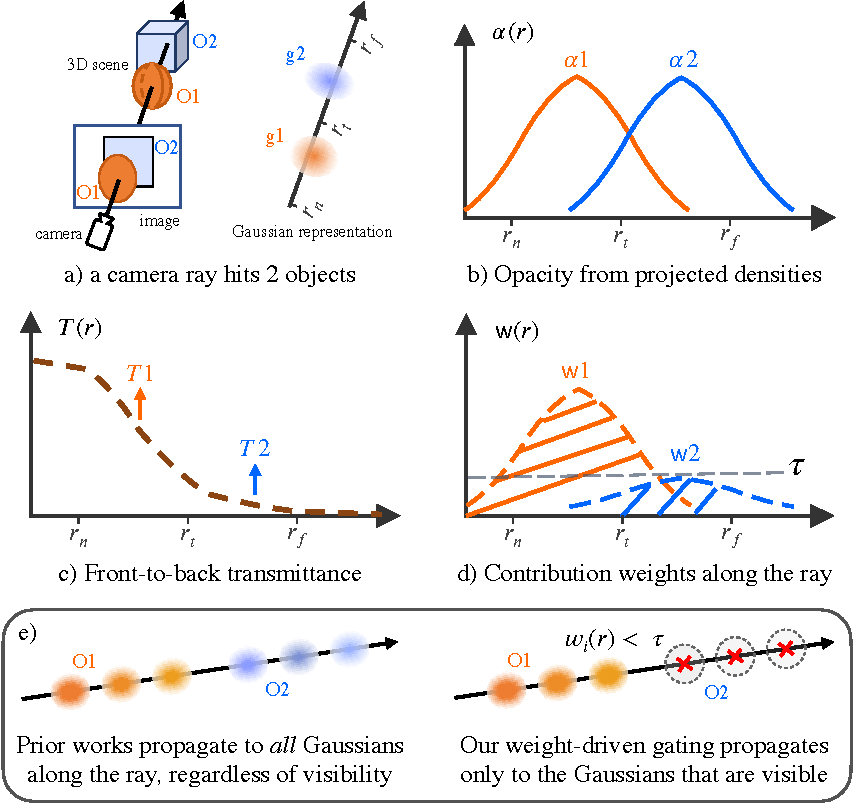
\includegraphics[width=0.95\linewidth]{figs/weight_driven_gating.pdf} % png/jpg/pdf 都行
  \caption{\textbf{Visibility-aware gating for semantic assignment} (Section~\ref{sec:gating}). Simplified representation of a scene with two objects (a) \(O_1,O_2\) and a camera ray \(r\) with Gaussians \(g_1,g_2\). We compute the opacity (b) and compute the transmittance front-to-back (c). Then we calculate the contribution weights for each ray, thresholding with $\tau$ (d). Instead of propagating the features to \textit{all} Gaussians as prior works do, our gating only propagates to the visible ones (e).}
% (b) Per-Gaussian opacity \(\alpha_i(r)\) from projected densities.
% (c) Front-to-back transmittance \(T_i(r)\).
% (d) Per-ray contribution weights \(w_i(r)=\alpha_i(r)\,T_i(r)\).
% (e) We apply a threshold \(\tau\) and supervise only Gaussians with \(w_i(r)\ge \tau\), preventing the classic ray-wise semantic misassignment (assigning the same 2D feature to all Gaussians along a ray) and improving multi-view consistency.
\vspace{-5mm}
  \label{fig:weight_driven_gating}
\end{figure}

% \noindent
\textbf{Ray Notation and Marginal Contributions.}
Let $r$ denote the camera ray through pixel $\mathbf{u}$. For brevity, we write
\begin{equation}
\label{eq:visibility_weights}
% more space in 2 lines (because the ID (9) would go in the new line)
\begin{aligned}
T_i(r) &\equiv T_i(\mathbf{u}), 
\quad\quad\quad\quad \alpha_i(r) \equiv \alpha_i(\mathbf{u}), \\
w_i(r) &\equiv \alpha_i(r)\,T_i(r).
\end{aligned}
% packed version all in 1 line including the ID
% \begin{alignedat}{3}
% T_i(r) &\equiv T_i(\mathbf{u}), \hspace{0.35em}&
% \alpha_i(r) &\equiv \alpha_i(\mathbf{u}), \hspace{0.35em}&
% w_i(r) &\equiv \alpha_i(r)\,T_i(r).
% \end{alignedat}
\end{equation}
where $\alpha_i(r)$ encodes \emph{coverage} (\ie, how much $g_i$ overlaps the pixel), $T_i(r)$ represents \emph{transmittance} (\ie, how much light reaches $g_i$ after occlusion by nearer Gaussians), and $w_i(r)$ measures how strongly $g_i$ influences the rendered sample along $r$. We name this as the \emph{Visibility} of a Gaussian from a specific view. Instead of assigning this feature to all Gaussians on the ray $r$, we use a two-stage visibility-aware gate (VAG).
We aggregate the weights into a per-view visibility score
\begin{equation}
% S_i^{s} \;=\; \sum_{\mathbf r\in\Omega_s} w_i^{s}(\mathbf r),
% \qquad
S_{\mathrm{tot}}^s \;=\; \sum\nolimits_{i, r} w_i(r) .
\label{eq:view_score}
\end{equation}

% \noindent
\textbf{Stage A: Mass Coverage on the Thresholded Set.}  
We sort $\{w_i(r)\}_i$ decreasingly, with the indices as $(1),\ldots,(k)$. 
We then retain the shortest prefix that accounts for a target fraction $\tau_{\mathrm{view}}\!\in\![0.5,0.75]$ of the total visibility mass:
\begin{equation}
k_{\mathrm{mass}}^\star
\,=\,
\min\Big\{k:\ \sum\nolimits_{j=1}^{k} w_{j} \ \ge\ \tau_{\mathrm{view}}\; S_{\mathrm{tot}}^{s} \Big\}.
\end{equation}
To suppress numerical noise, we apply a small absolute floor $\tau_{\mathrm{abs}}$ and define the candidate set as
\begin{equation}
\mathcal{G}_{\mathrm{mass}}^{s}
=
\Big\{ (1),\ldots,(k_{\mathrm{mass}}^\star) \Big\}
\ \cap\
\big\{ i:\ w_i \ge \tau_{\mathrm{abs}} \big\}.
\label{eq:mass_floor}
\end{equation}




\textbf{Stage B: Quantile-Constrained Truncation.}
Let $\tau_{q}^s=\mathrm{Quantile}_{1-q}(\{w_i\}_i)$, we define 
$K_q^{s}=|\{ i:\ w_i \ge \tau_{q}^s \}|$ and instead of imposing a separate hard limit, we determine the selection cap directly via the $q$-quantile as
%. Specifically,  set the final prefix length
\begin{equation}
\begin{aligned}
k_{\mathrm{keep}}^{\star} & = \min\!\big(k_{\mathrm{mass}}^\star,\; K_q^{s}\big), \\
% \quad
\mathcal G_{\mathrm{keep}}^{s} & = \big\{(1),\ldots,(k_{\mathrm{keep}}^{\star})\big\}.
\label{eq:quantile_truncate}
\end{aligned}
\end{equation}

\textbf{Why Mass \emph{then} Quantile?}
A fixed quantile alone tightly controls cardinality but ignores how visibility mass is distributed,
and under heavy tails may discard essential contributors.
Conversely, mass coverage secures a target fraction of visible content but can be liberal when scores are flat.
Our two-stage rule reconciles both: Stage~A guarantees coverage on the \emph{relevant} (floored) set,
while B imposes a quantile-derived \emph{cardinality constraint} $K_q^{s}$ that stabilizes scale across views.
Practically, if $K_q^{s}\!\ge\!k_{\mathrm{mass}}^\star$, we keep the mass-coverage set unchanged;
otherwise we truncate it to the top-$K_q^{s}$ by $w_i$.
The gate is thus \emph{coverage-faithful} and \emph{scale-adaptive}.

\subsection{Robust Multi-View Aggregation}
\label{sec:median}

\begin{table*}[t]
  \centering
  \setlength{\tabcolsep}{6.8pt}
  \begin{tabular}{c l cc*{4}{cc}}
    \toprule
    & &
    \multicolumn{2}{c}{\textbf{Mean}} &
    \multicolumn{2}{c}{Figurines} &
    \multicolumn{2}{c}{Ramen} &
    \multicolumn{2}{c}{Teatime} &
    \multicolumn{2}{c}{Waldo\_Kitchen} \\
    \cmidrule(lr){3-4} \cmidrule(lr){5-6} \cmidrule(lr){7-8}
    \cmidrule(lr){9-10} \cmidrule(lr){11-12}
    & Method & mIoU & mAcc & mIoU & mAcc & mIoU & mAcc & mIoU & mAcc & mIoU & mAcc \\
    %\midrule[1.1pt]
    % \rowcolor{gray!12}\multicolumn{12}{l}{\textbf{2D evaluation}}\\[-2pt]
    \midrule
    \multirow{8}{*}{\rotatebox{90}{2D evaluation}}
    & LERF~\cite{kerr2023lerf}          & 37.4 & 73.6 & 38.6 & 75.0 & 28.2 & 62.0 & 45.0 & 84.8 & 37.9 & 72.7 \\
    & LEGaussian~\cite{shi2024language} & 24.6 & 67.4 & 23.4 & 57.1 & 20.2 & 69.0 & 32.3 & 79.7 & 22.3 & 63.6 \\
    & GOI~\cite{goi2024}                & 42.0 & 59.2 & 23.9 & 44.6 & 33.7 & 56.3 & 55.8 & 67.8 & 54.5 & 68.2 \\
    & GAGS~\cite{peng2024gags}          & 54.1 & 81.7 & 53.6 & 78.6 & 46.8 & 69.0 & 60.3 & 88.1 & 55.8 & 90.9 \\
    & LangSplat~\cite{qin2024langsplat} & 51.4 & \nd84.3 & 44.7 & 80.4 & 51.2 & 73.2 & 65.1 & 88.1 & 44.5 & \fr95.5 \\
    & LangSplatV2~\cite{li2025langsplatv2}   & 59.9 & 84.1 & 56.4 & \nd82.1 & \fr51.8 & \nd74.7 & \fr72.2 & \fr93.2 & 59.1 & 86.4 \\
    & Occam's LGS~\cite{cheng2024occam}                     & \nd61.3 & 82.5 & \nd58.6 & 80.4 & 51.0 & 74.7 & 70.2 & \nd93.2 & \fr65.3 & 81.8 \\
    & \textbf{VALA [ours]}                         & \fr61.7 & \fr86.4 & \fr59.9 & \fr82.1 & \nd51.5 & \fr75.6 & \nd70.2 & 91.5 & \nd65.1 & \nd86.4 \\
    %\midrule[1.1pt]
    % \rowcolor{gray!12}\multicolumn{12}{l}{\textbf{3D evaluation}}\\[-2pt]
    \midrule
    \multirow{10}{*}{\rotatebox{90}{3D evaluation}}
    & LangSplat~\cite{qin2024langsplat} & 10.35 & 13.64 & 7.27 & 10.71 & 10.05 & 9.86 & 14.38 & 20.34 & 9.71 & 9.09 \\
    & LEGaussians~\cite{shi2024language}& 16.21 & 23.82 & 17.99 & 23.21 & 15.79 & 26.76 & 19.27 & 27.12 & 11.78 & 18.18 \\
    & OpenGaussian~\cite{wu2024opengaussian}
                                        & 38.36 & 51.43 & 39.29 & 55.36 & 31.01 & 42.25 & 60.44 & 76.27 & 22.70 & 31.82 \\
    & SuperGSeg~\cite{liang2024supergseg}
                                        & 35.94 & 52.02 & 43.68 & 60.71 & 18.07 & 23.94 & 55.31 & 77.97 & 26.71 & 45.45 \\
    & Dr.Splat~\cite{drsplat25}
                                        & 43.29 & 64.30 & 54.42 & 80.36 & 24.33 & 35.21 & 57.35 & 77.97 & 37.05 & 63.64 \\
    & InstanceGaussian~\cite{li2024instancegaussian}
                                        & 43.87 & 61.09 & 54.87 & 73.21 & 25.03 & 38.03 & 54.13 & 69.49 & 41.47 & 63.64 \\
    % & OpenGaussian~\cite{wu2024opengaussian}
    %                                     & 44.26 & 60.24 & 54.35 & 75.01 & 29.23 & 50.85 & 62.26 & 79.66 & 31.20 & 45.45 \\
    % & Dr.Splat~\cite{drsplat25} \TODO{check}        & 43.56 & 68.11 & 51.82 & 75.00 & 24.91 & 45.07 & 56.27 & 79.66 & 41.25 & 72.72 \\
    & CAGS~\cite{sun2025cags}           & \nd50.79 & 69.62 & 60.85 & 82.14 & 36.29 & 46.48 & \nd68.40 & 86.44 & 37.62 & 63.64 \\
    & VoteSplat~\cite{jiang2025votesplat}& 50.10 & 67.38 & \fr68.62 & \nd85.71 & \nd39.24 & \nd61.97 & 66.71 & 88.14 & 25.84 & 33.68 \\ 
    & Occam's LGS~\cite{cheng2024occam}& 47.22 & \nd74.84 & 52.90 & 78.57 & 32.01 & 54.92 & 61.02 & \fr93.22 & \nd42.95 & \nd72.72 \\
    & \textbf{VALA [ours]}                      & \fr58.02 & \fr82.85 & \nd60.38 & \fr89.29 & \fr45.41 & \fr67.61 & \fr70.61 & \nd88.14 & \fr55.71 & \fr86.36 \\
    \bottomrule
  \end{tabular}
  \vspace{-2mm}
    \caption{Comparison on LERF-OVS (mIoU / mAcc.). 
    In 3D, results are taken from~\cite{wu2024opengaussian,liang2024supergseg,drsplat25,sun2025cags,jiang2025votesplat} and otherwise evaluated by us.
    %$\dagger$ means the results reported in the corresponding paper; * means our implementation.
    }
    \vspace{-5mm}
    \label{tab:lerfovs}
\end{table*}

SAM+CLIP preprocessing pipelines~\cite{qin2024langsplat} yield crisp mask boundaries and per-pixel open-vocabulary embeddings, but their semantics are often viewpoint-dependent: changes in viewpoint and occlusion induce noticeable drift across views. To enforce multi-view consistency, several 3DGS-based methods first form 3D-consistent clusters, typically supervised with contrastive signals derived from SAM masks, and then assign a language embedding to each cluster~\cite{wu2024opengaussian, liang2024supergseg, li2024instancegaussian, piekenbrinck2025opensplat3d}. While this decoupled clustering can improve multi-view semantic consistency, it makes the pipelines' training multi-stage, thus prolonging the training time. More critically, because clustering is still driven by noisy, view-dependent 2D cues, it does not correct the root cause, namely, upstream semantic drift, which can bias the clusters and ultimately degrade the accuracy of the final language assignments.

To address this multi-view inconsistency at source, we adopt geometric median~\cite{martini1995torricelli, weiszfeld2008english, beck2015weiszfeld} to robustly aggregate multi-view features by minimizing the cosine distances in feature space. Unlike aggregation by weighted mean, it dampens view-dependent outliers and semantic drift.

\textbf{Weighted Euclidean Geometric Median.}
Using the visibility weights defined in Eq.~\eqref{eq:visibility_weights}, the (weighted) geometric median for $g_i$ is
\begin{equation}
\label{eq:gm_euclid}
\mathbf{z}_i^\star
=
\text{argmin}_{\mathbf{z}\in\mathbb{R}^d}
\;\sum\nolimits_{s} 
w_i(r)\,\bigl\lVert \mathbf{z} - \mathbf{f}_i^s \bigr\rVert .
\end{equation}

\textbf{Cosine-loss Median on the Unit Sphere.}
$\mathbf{f}(I,\mathbf{u})$ are $\ell_2$-normalized embeddings and thus angular consistency is most relevant. Therefore, we constrain $\mathbf{z}_i$ to the unit sphere $\mathbb{S}^{d-1}$ and minimize a weighted cosine loss:
\vspace{-3mm}
\begin{equation}
\label{eq:cosine_obj}
\mathbf{z}_i^\star 
\,=\, \text{argmin}_{\lVert \mathbf{z}\rVert_2=1}
\;\sum\nolimits_{s}
w_i(r)\,\bigl( 1 - \mathbf{f}_i^{s\top} \mathbf{z} \bigr),
\end{equation}
where $w_i(r)$ denotes the visibility weight of Gaussian $g_i$ from view $s$, since $r$ represents the view $s$.
The gradient of $\ell(\mathbf{f},\mathbf{z})=1-\mathbf{f}^\top\mathbf{z}$ on $\mathbb{S}^{d-1}$ is
\(
\nabla_{\mathbf{z}} \ell = -\bigl[\mathbf{f}-(\mathbf{f}^\top\mathbf{z})\,\mathbf{z}\bigr],
\)
the projection of $\mathbf{f}$ onto the tangent space at $\mathbf{z}$.
Compared to the Euclidean formulation in Eq.~\eqref{eq:gm_euclid}, this objective directly optimizes angular similarity, circumventing the scale sensitivity of Euclidean distances in high dimensions, where norm variations dominate over angular differences, and empirically leads to more stable 3D semantics (Table~\ref{tab:ablation_lerf}). 
% which avoids scale issues in high dimensions and empirically yields more stable 3D semantics.

% \vspace{-3mm}
\begin{algorithm}[t!]
\caption{Streaming cosine-loss median on $\mathbb{S}^{d-1}$ (Section~\ref{sec:median}).}
% \vspace{-3mm}
\label{alg:streaming_cosine_median}
\begin{algorithmic}[1]
\Require Stream $\{(\mathbf{f}_t, w_i^t)\}_{t=1}^T$ with $\mathbf{f}_t\in\mathbb{R}^d$, $\|\mathbf{f}_t\|_2=1$, and $w_i^t>0$
\State Initialize $\mathbf{z}_{i,0}\leftarrow \mathbf{f}_1$, \quad $W_{i,0}\leftarrow 0$
\For{$t=1,\ldots,T$}
    \State $\mathbf{d}_t \leftarrow \mathbf{f}_t - (\mathbf{f}_t^\top \mathbf{z}_{i,t})\,\mathbf{z}_{i,t}$ \Comment{tangent direction}
    \State $\eta_t \leftarrow \dfrac{w_i^t}{W_{i,t}+w_i^t}$ \Comment{streaming step size}
    \State $\mathbf{z}_{i,t+1} \leftarrow \mathrm{Norm}\!\big(\mathbf{z}_{i,t} + \eta_t\,\mathbf{d}_t\big)$
    \State $W_{i,t+1} \leftarrow W_{i,t} + w_i^t$
\EndFor
\State \Return $\mathbf{z}_i \leftarrow \mathbf{z}_{i,T}$, \ $W_i \leftarrow W_{i,T}$
% \vspace{-5mm}
\end{algorithmic}
% \vspace{-5mm}
\end{algorithm}
% \vspace{-1mm}


% \noindent
\textbf{Constant-Memory Streaming Update.} 
While effective, solving Eq.~\eqref{eq:cosine_obj} with the classical Weiszfeld algorithm~\cite{eckhardt1980weber} requires repeated full-batch updates over all Gaussian features, which scales linearly with the number of views and becomes computationally prohibitive in practice. 
To address this, we adopt a constant-memory streaming scheme inspired by online optimization~\cite{kirillov2023sam}.
Specifically, as detailed in Algorithm~\ref{alg:streaming_cosine_median}, we maintain only the current estimate $(\mathbf{z}_{i,t},W_{i,t})$, where $W_{i,t}$ is the cumulative visibility weight, and incorporate each new observation $(\mathbf{f}_t,w_i^t)$ via
\vspace{-1mm}
\begin{align}
\mathbf{z}_{i,t+1}
&= \mathrm{Norm}\!\left(
\mathbf{z}_{i,t}
+\eta_t\, w_i^t\,
\bigl[\mathbf{f}_t - (\mathbf{f}_t^\top \mathbf{z}_{i,t})\,\mathbf{z}_{i,t}\bigr]
\right), \\
\eta_t &= \frac{w_i^t}{W_{i,t}+w_i^t}\,, \qquad
W_{i,t+1} = W_{i,t} + w_i^t,
\vspace{-2mm}
\end{align}

% where $\mathrm{Norm}(\mathbf{x})=\mathbf{x}/\|\mathbf{x}\|_2$ ensures $\mathbf{z}_{i,t}\in\mathbb{S}^{d-1}$ at every step.
% The direction $\mathbf{f}_t-(\mathbf{f}_t^\top \mathbf{z}_{i,t})\mathbf{z}_{i,t}$ corresponds to the tangent component that increases cosine similarity, while the adaptive step size $\eta_t$ ensures each sample contributes proportionally to its visibility.
% Under standard stochastic approximation assumptions (bounded variance and diminishing step sizes), $\mathbf{z}_{i,t}$ converges to a stationary point of Eq.~\eqref{eq:cosine_obj} at rate $\mathcal{O}(1/\sqrt{W_{i,t}})$.
where $\mathrm{Norm}(\mathbf{x})=\mathbf{x}/\|\mathbf{x}\|_2$ projects $\mathbf{z}_{i,t}$ onto the unit sphere $\mathbb{S}^{d-1}$.
The update direction $\mathbf{f}_t-(\mathbf{f}_t^\top \mathbf{z}_{i,t})\mathbf{z}_{i,t}$ lies in the tangent space and increases cosine similarity, while the adaptive step size $\eta_t$ weights each sample according to its visibility.
Under standard stochastic approximation assumptions, $\mathbf{z}_{i,t}$ converges to a stationary point of Eq.~\eqref{eq:cosine_obj} at rate $\mathcal{O}(1/\sqrt{W_{i,t}})$.

